\documentclass[aspectratio=169, 11pt]{beamer}

% Packages
\usepackage[utf8]{inputenc}
\usepackage{amsmath, amssymb, amsfonts}
\usepackage{graphicx}
\usepackage{booktabs}
\usepackage{ragged2e}
\usepackage{minted}
\usepackage{xcolor}
\usepackage{tikz}
\usepackage{algorithm}
\usepackage{algorithmic}
\usepackage{listings}
\usepackage{tcolorbox}

\usetikzlibrary{arrows.meta,positioning,fit,shapes.symbols}
\usetikzlibrary{arrows,shapes}
\definecolor{LightGray}{gray}{0.975}
\definecolor{links}{HTML}{2A1B81}
\hypersetup{colorlinks,linkcolor=,urlcolor=blue}
\AtBeginEnvironment{minted}{%
    \renewcommand{\fcolorbox}[4][]{#4}
}

\title[FP]{ML101 \\ Chapter 4: Frequent Patterns}
\subtitle{Data Mining: Concepts and Techniques}
\author{Jiawei Han, Jian Pei \& Hanghang Tong}
\date{\today}

% Remove navigation symbols
\setbeamertemplate{navigation symbols}{}

\defbeamertemplate*{footline}{shadow theme}{
    \leavevmode
    \hbox{
        \begin{beamercolorbox}[
                wd =        0.33\paperwidth,
                ht =        2.5ex,
                dp =        1.125ex,
                leftskip =  0.3cm plus1fil,
                rightskip = 0.3cm
            ]{author in head/foot}
            \flushleft ML101
        \end{beamercolorbox}
        \begin{beamercolorbox}[
                wd =        0.33\paperwidth,
                ht =        2.5ex,
                dp =        1.125ex,
                leftskip =  0.3cm plus1fil,
                rightskip = 0.3cm
            ]{author in head/foot}
            \insertshorttitle
        \end{beamercolorbox}
        \begin{beamercolorbox}[
                wd =        0.33\paperwidth,
                ht =        2.5ex,
                dp =        1.125ex,
                leftskip =  0.3cm plus1fil,
                rightskip = 0.3cm
            ]{title in head/foot}
            \hfill \insertframenumber\,/\,\inserttotalframenumber%
        \end{beamercolorbox}
    }
}

\AtBeginSection[]
{
     \begin{frame}<beamer>
     \frametitle{Plan}
     \tableofcontents[currentsection]
     \end{frame}
}

\usefonttheme{serif}

\newcommand\Wider[2][18mm]{%
    \makebox[\linewidth][c]{%
        \begin{minipage}{\dimexpr\textwidth+#1\relax}
            \raggedright#2
        \end{minipage}%
    }%
}
\newcommand\userinput[1]{\textbf{#1}}

\begin{document}

\frame{\titlepage}

\begin{frame}{Data Mining: Concepts and Techniques}
    \centering
    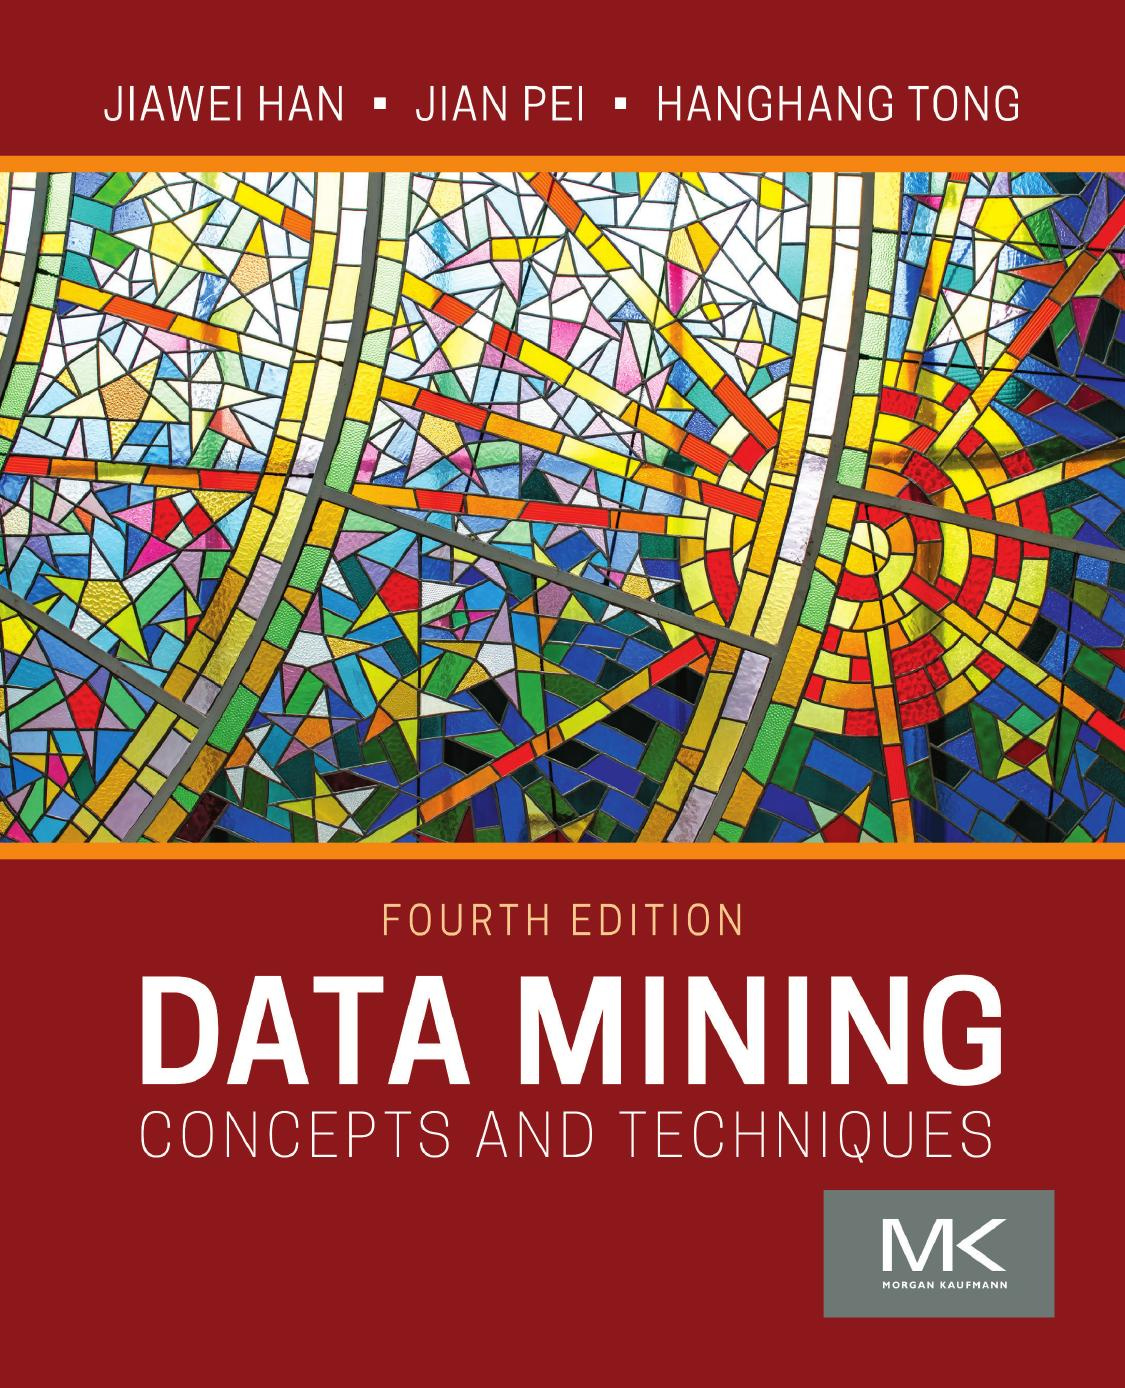
\includegraphics[height=0.7\textheight]{figures/cover} \\
    \vspace{4mm}
    {
        \tiny
        Content has been extracted from \textit{Data Mining: Concepts and Techniques}, Fourth Edition, by Jiawei Han, Jian Pei \& Hanghang Tong. Morgan Kaufmann Publishers. 2023.\\
        Visit \url{https://hanj.cs.illinois.edu/bk4/}.\\
    }
\end{frame}

\begin{frame}{What Are Patterns?}
    \begin{itemize}
        \item \textbf{What are patterns?}
        \begin{itemize}
            \item \textbf{Patterns:} A set of items, subsequences, or substructures that occur frequently together (or strongly correlated) in a data set
            \item Patterns represent intrinsic and important properties of datasets
        \end{itemize}
    \end{itemize}
    \vspace{5mm}
    \centering
    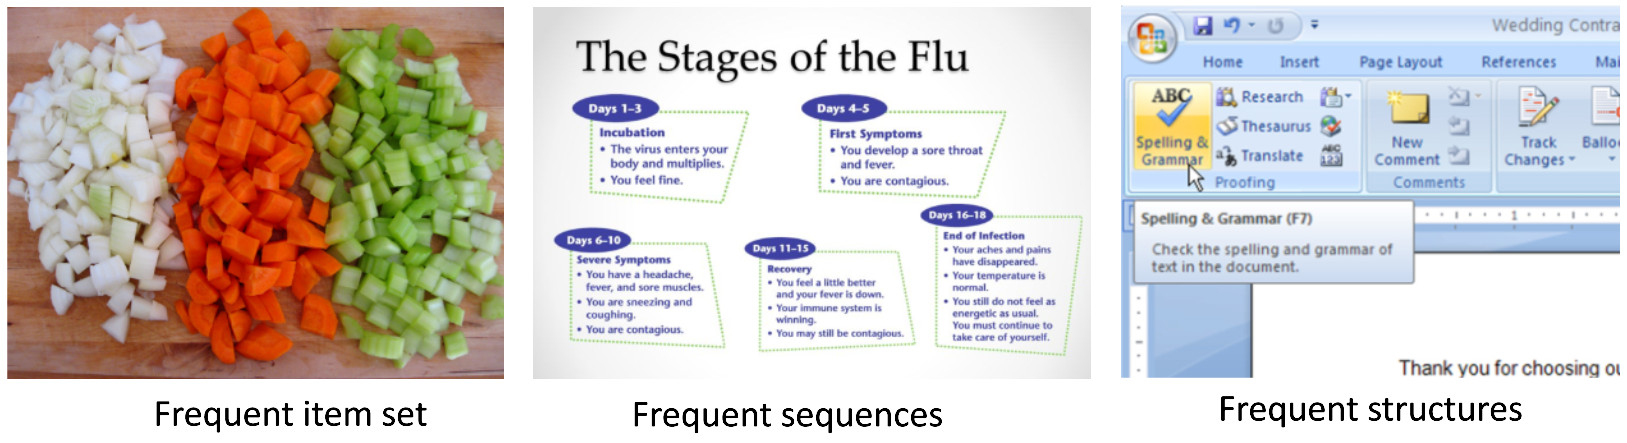
\includegraphics[width=\textwidth]{figures/examples}
\end{frame}

\section{Basic Concepts}

\begin{frame}{What Is Pattern Discovery?}
    \begin{columns}[T]
        \begin{column}{0.52\textwidth}
            \begin{itemize}
                \item \textbf{Pattern discovery:} Uncovering patterns from massive data sets
                \item It can answer questions such as:
                \begin{itemize}
                    \item What products were often purchased together?
                    \item What are the subsequent purchases after buying an iPad?
                \end{itemize}
            \end{itemize}
        \end{column}
        \begin{column}{0.46\textwidth}
            \centering
            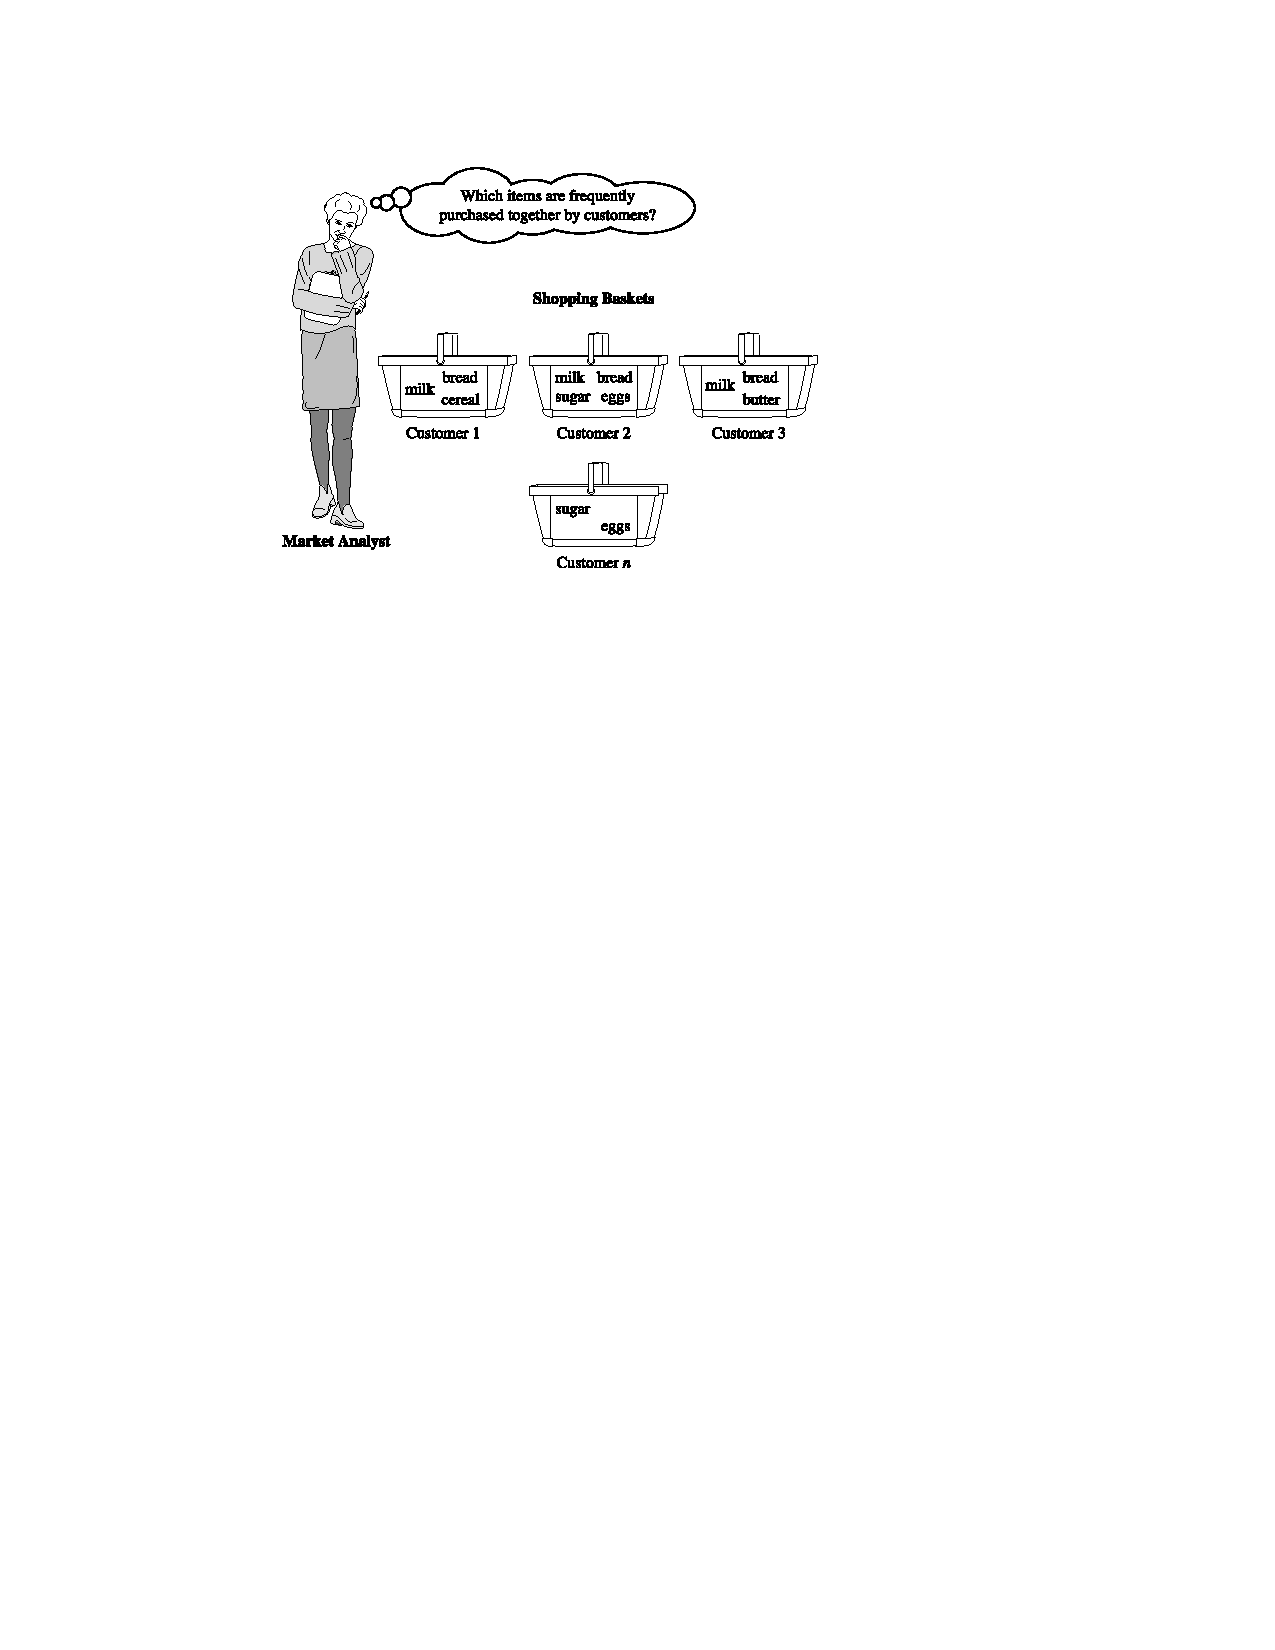
\includegraphics[width=\textwidth]{figures/4_2}
        \end{column}
    \end{columns}
\end{frame}

\begin{frame}{Pattern Discovery: Why Is It Important?}
    \begin{itemize}
        \item \textbf{Foundation for many essential data mining tasks}
        \begin{itemize}
            \item Association, correlation, and causality analysis
            \item Mining sequential, structural (e.g., sub-graph) patterns
            \item Classification: Discriminative pattern-based analysis
            \item Cluster analysis: Pattern-based subspace clustering
        \end{itemize}
        \vspace{2mm}
        \item \textbf{Broad applications}
        \begin{itemize}
            \item Market basket analysis, cross-marketing, catalog design, sale campaign analysis, Web log analysis, biological sequence analysis
            \item Many types of data: spatiotemporal, multimedia, time-series, and stream data
        \end{itemize}
    \end{itemize}
\end{frame}

\begin{frame}{Basic Concepts: Transactional Database}
    \begin{itemize}
        \item Let $I = \{I_1, I_2, \dots, I_m\}$ be a set of items
        \item \textbf{Transactional Database (TDB)}
        \begin{itemize}
            \item Each transaction is associated with an identifier, called a \textbf{TID}.
            \item May also have counts associated with each item sold
        \end{itemize}
    \end{itemize}
    \vspace{3mm}
    \centering
    \begin{tabular}{cl}
        \toprule
        \textbf{Tid} & \textbf{Items bought} \\
        \midrule
        1 & Beer, Nuts, Diaper \\
        2 & Beer, Coffee, Diaper \\
        3 & Beer, Diaper, Eggs \\
        4 & Nuts, Eggs, Milk \\
        5 & Nuts, Coffee, Diaper, Eggs, Milk \\
        \bottomrule
    \end{tabular}
\end{frame}

\begin{frame}{Basic Concepts: $k$-Itemsets and Their Supports}
    \begin{columns}[T]
        \begin{column}{0.49\textwidth}
            \small
            \begin{itemize}
                \item \textbf{Itemset:} A set of one or more items
                \item \textbf{$k$-itemset:} An itemset containing $k$ items:
                $$X = \{x_1, \dots, x_k\}$$
                \begin{itemize}
                    \item Ex.\ $\{\text{Beer, Nuts, Diaper}\}$ is a 3-itemset
                \end{itemize}
                \item \textbf{Absolute support (count)}
                \begin{itemize}
                    \item $\sup\{X\} =$ occurrences of an itemset $X$
                    \item Ex.\ $\sup\{\text{Beer}\} = 3$, $\sup\{\text{Diaper}\} = 4$
                    \item Ex.\ $\sup\{\text{Beer, Diaper}\} = 3$
                    \item Ex.\ $\sup\{\text{Beer, Eggs}\} = 1$
                \end{itemize}
            \end{itemize}
        \end{column}
        \begin{column}{0.49\textwidth}
            \centering
            \footnotesize
            \begin{tabular}{cl}
                \toprule
                \textbf{Tid} & \textbf{Items bought} \\
                \midrule
                1 & Beer, Nuts, Diaper \\
                2 & Beer, Coffee, Diaper \\
                3 & Beer, Diaper, Eggs \\
                4 & Nuts, Eggs, Milk \\
                5 & Nuts, Coffee, Diaper, Eggs, Milk \\
                \bottomrule
            \end{tabular}
            \vspace{4mm}
            \begin{itemize}
                \item \textbf{Relative support (\%)}
                \begin{itemize}
                    \item $s\{X\} =$ The fraction of transactions that contains $X$ (i.e., the \textbf{probability} that a transaction contains $X$)
                    \item Ex.\ $s\{\text{Beer}\} = 3/5 = 60\%$
                    \item Ex.\ $s\{\text{Diaper}\} = 4/5 = 80\%$
                    \item Ex.\ $s\{\text{Beer, Eggs}\} = 1/5 = 20\%$
                \end{itemize}
            \end{itemize}
        \end{column}
    \end{columns}
\end{frame}

\begin{frame}{Basic Concepts: Frequent Itemsets (Patterns)}
    \begin{columns}[T]
        \begin{column}{0.49\textwidth}
            \small
            \begin{itemize}
                \item An itemset (or a pattern) $X$ is \textbf{frequent} if the support of $X$ is no less than a $\text{minsup}$ threshold $\sigma$
                \item Let $\sigma = 50\%$ ($\sigma$: $\text{minsup}$ threshold) for the given 5-transaction dataset:
                \begin{itemize}
                    \item \textbf{All the frequent 1-itemsets:}
                    \begin{itemize}
                        \item Beer: $3/5$ ($60\%$); Nuts: $3/5$ ($60\%$); Diaper: $4/5$ ($80\%$); Eggs: $3/5$ ($60\%$)
                    \end{itemize}
                    \item \textbf{All the frequent 2-itemsets:}
                    \begin{itemize}
                        \item $\{\text{Beer, Diaper}\}$: $3/5$ ($60\%$)
                    \end{itemize}
                    \item \textbf{All the frequent 3-itemsets?}
                    \begin{itemize}
                        \item None
                    \end{itemize}
                \end{itemize}
            \end{itemize}
        \end{column}
        \begin{column}{0.49\textwidth}
            \centering
            \footnotesize
            \begin{tabular}{cl}
                \toprule
                \textbf{Tid} & \textbf{Items bought} \\
                \midrule
                1 & Beer, Nuts, Diaper \\
                2 & Beer, Coffee, Diaper \\
                3 & Beer, Diaper, Eggs \\
                4 & Nuts, Eggs, Milk \\
                5 & Nuts, Coffee, Diaper, Eggs, Milk \\
                \bottomrule
            \end{tabular}
            \vspace{2mm}
            \small
            \begin{itemize}
                \item Why do these itemsets (shown on the left) form the complete set of frequent $k$-itemsets (patterns) for any $k$?
                \item \textbf{Observation:} We may need an efficient method to mine a complete set of frequent patterns
            \end{itemize}
        \end{column}
    \end{columns}
\end{frame}

\begin{frame}{From Frequent Itemsets to Association Rules}
    \begin{itemize}
        \item Compared with itemsets, \textbf{association rules} can be more telling
        \begin{itemize}
            \item Ex.\ $\text{Diaper} \rightarrow \text{Beer}$: Buying diapers may likely lead to buying beers
        \end{itemize}
        \item Note: $X \cup Y$: the union of two itemsets
        \begin{itemize}
            \item The set contains both $X$ and $Y$
            \item $\{\text{Beer}\} \cup \{\text{Diaper}\} = \{\text{Beer, Diaper}\}$
        \end{itemize}
    \end{itemize}
    \vspace{2mm}
    \centering
    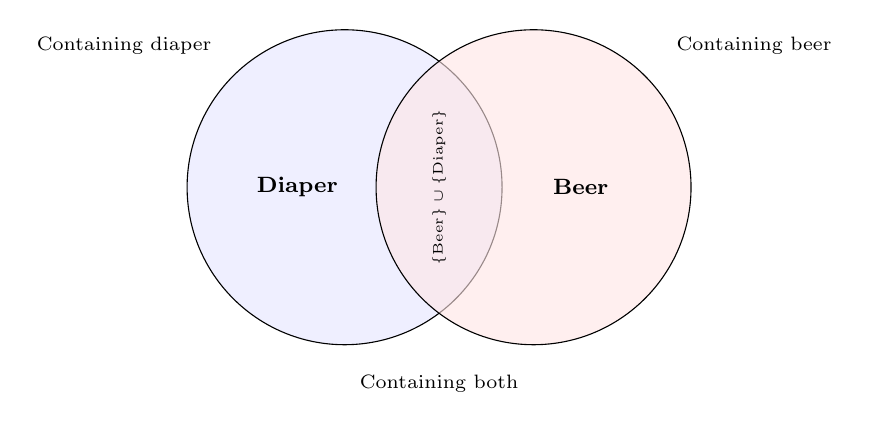
\begin{tikzpicture}[scale=1]
        \draw[fill=blue!10, fill opacity=0.6] (-1.2,0) circle (2cm);
        \draw[fill=red!10, fill opacity=0.6] (1.2,0) circle (2cm);
        \node at (-1.8,0) {\footnotesize \textbf{Diaper}};
        \node at (1.8,0) {\footnotesize \textbf{Beer}};
        \node[rotate=90] at (0,0) {\tiny $\{\text{Beer}\} \cup \{\text{Diaper}\}$};
        \node at (-4,1.8) {\scriptsize Containing diaper};
        \node at (0,-2.5) {\scriptsize Containing both};
        \node at (4,1.8) {\scriptsize Containing beer};
    \end{tikzpicture}
\end{frame}

\begin{frame}{Association Rules}
    \begin{columns}[T]
        \begin{column}{0.58\textwidth}
            \footnotesize
            \begin{itemize}
                \item How do we compute the strength of an association rule $X \rightarrow Y$ (Both $X$ and $Y$ are itemsets)?
                \item We first compute the following two metrics, $s$ and $c$:
                \begin{itemize}
                    \item \textbf{Support} of $X \cup Y$:
                    \begin{itemize}
                        \item Ex.\ $s\{\text{Diaper, Beer}\} = 3/5 = 0.6$ (i.e., $60\%$)
                    \end{itemize}
                    \item \textbf{Confidence} of $X \rightarrow Y$:
                    \begin{itemize}
                        \item The conditional probability that a transaction containing $X$ also contains $Y$:
                        $$c = \frac{\sup(X, Y)}{\sup(X)}$$
%                         \item Ex.\ $c = \frac{\sup\{\text{Diaper, Beer}\}}{\sup\{\text{Diaper}\}} = \frac{3}{4} = 0.75$
                     \end{itemize}
                \end{itemize}
            \end{itemize}
        \end{column}
        \begin{column}{0.40\textwidth}
            \centering
            \footnotesize
            \begin{tabular}{cl}
                \toprule
                \textbf{Tid} & \textbf{Items bought} \\
                \midrule
                1 & Beer, Nuts, Diaper \\
                2 & Beer, Coffee, Diaper \\
                3 & Beer, Diaper, Eggs \\
                4 & Nuts, Eggs, Milk \\
                5 & Nuts, Coffee, Diaper, Eggs, Milk \\
                \bottomrule
            \end{tabular}
            \vspace{7mm}
            \begin{itemize}
                \item Ex.\ $c = \frac{\sup\{\text{Diaper, Beer}\}}{\sup\{\text{Diaper}\}} = \frac{3}{4} = 0.75$
            \end{itemize}
        \end{column}
    \end{columns}
    \vspace{2mm}
    \small
    \begin{itemize}
        \item In pattern analysis, we are often interested in those rules that dominate the database, and these two metrics ensure the \textbf{popularity} and \textbf{correlation} of $X$ and $Y$.
    \end{itemize}
\end{frame}

\begin{frame}{Mining Frequent Itemsets and Association Rules}
    \begin{columns}[T]
        \begin{column}{0.58\textwidth}
            \small
            \begin{itemize}
                \item \textbf{Association rule mining}
                \begin{itemize}
                    \item Given two thresholds: $\text{minsup}$, $\text{minconf}$
                    \item Find all of the rules, $X \rightarrow Y\ (s, c)$ such that $s \ge \text{minsup}$ and $c \ge \text{minconf}$
                \end{itemize}
                \item Let $\text{minsup} = 50\%$
                \begin{itemize}
                    \item Freq.\ 1-itemsets: Beer: 3, Nuts: 3, Diaper: 4, Eggs: 3
                    \item Freq.\ 2-itemsets: $\{\text{Beer, Diaper}\}$: 3
                \end{itemize}
                \item Let $\text{minconf} = 50\%$
                \begin{itemize}
                    \item $\text{Beer} \rightarrow \text{Diaper}\ (60\%, 100\%)$
                    \item $\text{Diaper} \rightarrow \text{Beer}\ (60\%, 75\%)$
                    \item \textit{(Q: Are these all the rules satisfying the two conditions?)}
                \end{itemize}
            \end{itemize}
        \end{column}
        \begin{column}{0.40\textwidth}
            \centering
            \footnotesize
            \begin{tabular}{cl}
                \toprule
                \textbf{Tid} & \textbf{Items bought} \\
                \midrule
                1 & Beer, Nuts, Diaper \\
                2 & Beer, Coffee, Diaper \\
                3 & Beer, Diaper, Eggs \\
                4 & Nuts, Eggs, Milk \\
                5 & Nuts, Coffee, Diaper, Eggs, Milk \\
                \bottomrule
            \end{tabular}
            \vspace{2mm}
            \small
            \begin{itemize}
                \item \textbf{Observations:}
                \begin{itemize}
                    \item Mining association rules and mining frequent patterns are very close problems
                    \item Scalable methods are needed for mining large datasets
                \end{itemize}
            \end{itemize}
        \end{column}
    \end{columns}
\end{frame}

\begin{frame}{Challenge: There Are Too Many Frequent Patterns!}
    \small
    \begin{itemize}
        \item A long pattern contains a combinatorial number of sub-patterns
        \item How many frequent itemsets does the following $\text{TDB}_1$ contain ($\text{minsup} = 1$)?
        \begin{itemize}
            \item $\text{TDB}_1$: $T_1: \{a_1, \dots, a_{50}\}$; \quad $T_2: \{a_1, \dots, a_{100}\}$
        \end{itemize}
        \item Let's have a try:
        \begin{itemize}
            \item 1-itemsets: $\{a_1\}: 2, \{a_2\}: 2, \dots, \{a_{50}\}: 2, \{a_{51}\}: 1, \dots, \{a_{100}\}: 1$
            \item 2-itemsets: $\{a_1, a_2\}: 2, \dots, \{a_1, a_{50}\}: 2, \{a_1, a_{51}\}: 1, \dots, \{a_{99}, a_{100}\}: 1$
            \item $\dots$
            \item 99-itemsets: $\{a_1, a_2, \dots, a_{99}\}: 1, \dots, \{a_2, a_3, \dots, a_{100}\}: 1$
            \item 100-itemset: $\{a_1, a_2, \dots, a_{100}\}: 1$
        \end{itemize}
        \item The total number of frequent itemsets:
        $$\binom{100}{1} + \binom{100}{2} + \dots + \binom{100}{100} = 2^{100} - 1 \approx 1.27 \times 10^{30}$$
        \item \textbf{A too huge set for any one to compute or store!}
    \end{itemize}
\end{frame}

\begin{frame}{Expressing Patterns in Compressed Form: Closed Patterns}
    \begin{itemize}
        \item \textbf{How to handle such a challenge?}
        \item \textbf{Solution 1: Closed patterns:} A pattern (itemset) $X$ is \textbf{closed} if $X$ is frequent, and there exists no super-pattern $Y \supset X$, with the same support as $X$
        \item Let Transaction DB $\text{TDB}_1$: $T_1: \{a_1, \dots, a_{50}\}$; \quad $T_2: \{a_1, \dots, a_{100}\}$
        \item Suppose $\text{minsup} = 1$. How many closed patterns does $\text{TDB}_1$ contain?
        \begin{itemize}
            \item \textbf{Two:} $P_1$: ``$\{a_1, \dots, a_{50}\}: 2$''; \quad $P_2$: ``$\{a_1, \dots, a_{100}\}: 1$''
        \end{itemize}
        \item \textbf{Closed pattern is a lossless compression of frequent patterns}
        \begin{itemize}
            \item Reduces the \# of patterns but does not lose the support information!
            \item You will still be able to say: ``$\{a_2, \dots, a_{40}\}: 2$'', ``$\{a_5, a_{51}\}: 1$''
        \end{itemize}
    \end{itemize}
\end{frame}

\begin{frame}{Expressing Patterns in Compressed Form: Max-Patterns}
    \begin{itemize}
        \item \textbf{Solution 2: Max-patterns:} A pattern $X$ is a \textbf{max-pattern} if $X$ is frequent and there exists no frequent super-pattern $Y \supset X$
        \item \textbf{Difference from closed-patterns?}
        \begin{itemize}
            \item Do not care the real support of the sub-patterns of a max-pattern
        \end{itemize}
        \item Let Transaction DB $\text{TDB}_1$: $T_1: \{a_1, \dots, a_{50}\}$; \quad $T_2: \{a_1, \dots, a_{100}\}$
        \item Suppose $\text{minsup} = 1$. How many max-patterns does $\text{TDB}_1$ contain?
        \begin{itemize}
            \item \textbf{One:} $P$: ``$\{a_1, \dots, a_{100}\}: 1$''
        \end{itemize}
        \item \textbf{Max-pattern is a lossy compression!}
        \begin{itemize}
            \item We only know $\{a_1, \dots, a_{40}\}$ is frequent
            \item But we do not know the real support of $\{a_1, \dots, a_{40}\}, \dots,$ any more!
        \end{itemize}
        \item Thus in many applications, mining closed-patterns is more desirable than mining max-patterns
    \end{itemize}
\end{frame}

\section{Frequent Itemset Mining Methods}

\begin{frame}{Efficient Pattern Mining Methods}
    \begin{itemize}
        \item The Downward Closure Property of Frequent Patterns
        \begin{itemize}
            \item The Apriori Algorithm
            \item Extensions or Improvements of Apriori
        \end{itemize}
        \item Mining Frequent Patterns by Exploring Vertical Data Format
        \item FPGrowth: A Frequent Pattern-Growth Approach
        \item Mining Closed Patterns
    \end{itemize}
\end{frame}

\subsection{Apriori}

\begin{frame}{The Downward Closure Property of Frequent Patterns}
    \begin{itemize}
        \item \textbf{Observation:} From $\text{TDB}_1$: $T_1: \{a_1, \dots, a_{50}\}$; \quad $T_2: \{a_1, \dots, a_{100}\}$
        \begin{itemize}
            \item We get a frequent itemset: $\{a_1, \dots, a_{50}\}$
            \item Also, its subsets are all frequent: $\{a_1\}, \{a_2\}, \dots, \{a_{50}\}, \{a_1, a_2\}, \dots, \{a_1, \dots, a_{49}\}, \dots$
            \item There are some hidden relationships among frequent patterns!
        \end{itemize}
        \item The \textbf{downward closure (also called ``Apriori'')} property of frequent patterns:
        \begin{itemize}
            \item If $\{\text{\textbf{beer, diaper, nuts}}\}$ is frequent, so is $\{\text{\textbf{beer, diaper}}\}$
            \item Every transaction containing $\{\text{beer, diaper, nuts}\}$ also contains $\{\text{beer, diaper}\}$
            \item \textbf{Apriori: Any subset of a frequent itemset must be frequent}.
        \end{itemize}
        \item \textbf{Efficient mining methodology}
        \begin{itemize}
            \item If any subset of an itemset $S$ is infrequent, then there is no chance for $S$ to be frequent, why do we even have to consider $S$!? \textbf{A sharp knife for pruning!}
        \end{itemize}
    \end{itemize}
\end{frame}

\begin{frame}{Apriori Pruning and Scalable Mining Methods}
    \begin{itemize}
        \item \textbf{Apriori pruning principle:} If there is any itemset which is infrequent, its superset should not even be generated! (Agrawal \& Srikant @VLDB'94, Mannila, et al.\ @KDD'94)
        \vspace{3mm}
        \item \textbf{Scalable mining Methods: Three major approaches}
        \begin{itemize}
            \item \textbf{Level-wise, join-based approach:} Apriori (Agrawal \& Srikant @VLDB'94)
            \item \textbf{Vertical data format approach:} Eclat (Zaki, Parthasarathy, Ogihara, Li @KDD'97)
            \item \textbf{Frequent pattern projection and growth:} FPGrowth (Han, Pei, Yin @SIGMOD'00)
        \end{itemize}
    \end{itemize}
\end{frame}

\begin{frame}{Apriori: A Candidate Generation \& Test Approach}
    \begin{itemize}
        \item \textbf{Outline of Apriori (level-wise, candidate generation and test)}
        \begin{itemize}
            \item Scan DB once to get frequent 1-itemset
            \item \textbf{Repeat}
            \begin{itemize}
                \item Generate length-$(k+1)$ candidate itemsets from length-$k$ frequent itemsets
                \item Test the candidates against DB to find frequent $(k+1)$-itemsets
                \item Set $k := k + 1$
            \end{itemize}
            \item \textbf{Until} no frequent or candidate set can be generated
            \item Return all the frequent itemsets derived
        \end{itemize}
    \end{itemize}
\end{frame}

\begin{frame}{The Apriori Algorithm (Pseudo-Code)}
    \begin{itemize}
        \item $C_k$: Candidate itemset of size $k$
        \item $F_k$: Frequent itemset of size $k$
    \end{itemize}
    \vspace{2mm}
    \begin{tcolorbox}[colback=LightGray, colframe=black!30, title=\textbf{Apriori Algorithm}]
        \footnotesize
        \texttt{$k := 1$;}\\
        \texttt{$F_k := \{\text{frequent items}\}$; \hfill // frequent 1-itemset}\\
        \texttt{\textbf{While} ($F_k \neq \emptyset$) \textbf{do} \{ \hfill // when $F_k$ is non-empty}\\
        \texttt{\hspace*{6mm}$C_{k+1} := \text{candidates generated from } F_k$; \hfill // candidate generation}\\
        \texttt{\hspace*{6mm}Derive $F_{k+1}$ by counting candidates in $C_{k+1}$ with respect to TDB at $\text{minsup}$;}\\
        \texttt{\hspace*{6mm}$k := k + 1$;}\\
        \texttt{\}}\\
        \texttt{\textbf{return} $\bigcup_k F_k$; \hfill // return $F_k$ generated at each level}
    \end{tcolorbox}
\end{frame}

\begin{frame}{Apriori: Implementation Tricks}
    \begin{columns}[T]
        \begin{column}{0.55\textwidth}
            \begin{itemize}
                \item \textbf{How to generate candidates?}
                \begin{itemize}
                    \item Step 1: self-joining $F_k$
                    \item Step 2: pruning
                \end{itemize}
                \item \textbf{Example of candidate-generation}
                \begin{itemize}
                    \item $F_3 = \{abc, abd, acd, ace, bcd\}$
                    \item \textbf{Self-joining:} $F_3 * F_3$
                    \begin{itemize}
                        \item $abcd$ from $abc$ and $abd$
                        \item $acde$ from $acd$ and $ace$
                    \end{itemize}
                    \item \textbf{Pruning:}
                    \begin{itemize}
                        \item $acde$ is removed because $ade$ is not in $F_3$
                    \end{itemize}
                    \item $C_4 = \{abcd\}$
                \end{itemize}
            \end{itemize}
        \end{column}
        \begin{column}{0.44\textwidth}
            \centering
            \vspace{4mm}
            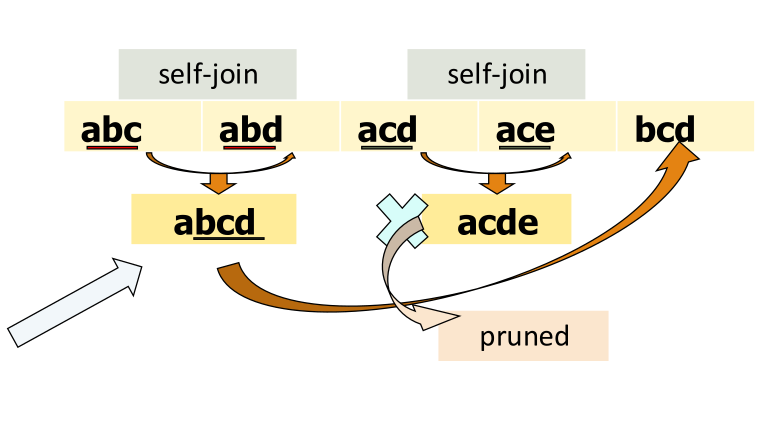
\includegraphics[width=\textwidth]{figures/prune} \\
            \footnotesize
            \textit{prefix matching}
        \end{column}
    \end{columns}
\end{frame}

\begin{frame}{Candidate Generation (Pseudo-Code)}
    \centering
    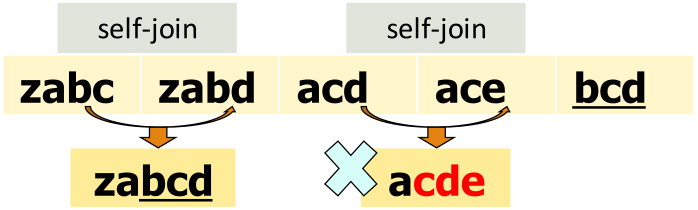
\includegraphics[width=0.3\textwidth]{figures/prefix_matching}
    \begin{itemize}
        \item Suppose the items in $F_{k-1}$ are listed in an order
    \end{itemize}
    \begin{tcolorbox}[colback=LightGray, colframe=black!30, title=\textbf{Candidate generation}]
        \footnotesize
        \texttt{// Step 1: Joining}\\
        \texttt{\textbf{for each} $p$ \textbf{in} $F_{k-1}$}\\
        \texttt{\hspace*{4mm}\textbf{for each} $q$ \textbf{in} $F_{k-1}$}\\
        \texttt{\hspace*{8mm}\textbf{if} $p.\text{item}_1 = q.\text{item}_1, \dots, p.\text{item}_{k-2} = q.\text{item}_{k-2},$}\\
        \texttt{\hspace*{11mm}$p.\text{item}_{k-1} < q.\text{item}_{k-1}$ \{}\\
        \texttt{\hspace*{12mm}$c = \text{join}(p, q)$}\\
        \texttt{\hspace*{12mm}// Step 2: pruning}\\
        \texttt{\hspace*{12mm}\textbf{if} $\text{has\_infrequent\_subset}(c, F_{k-1})$}\\
        \texttt{\hspace*{16mm}\textbf{continue} \hfill // prune}\\
        \texttt{\hspace*{12mm}\textbf{else} add $c$ to $C_k$}\\
        \texttt{\hspace*{8mm}\}}
    \end{tcolorbox}
\end{frame}

\begin{frame}{The Apriori Algorithm --An Example}
    \centering
    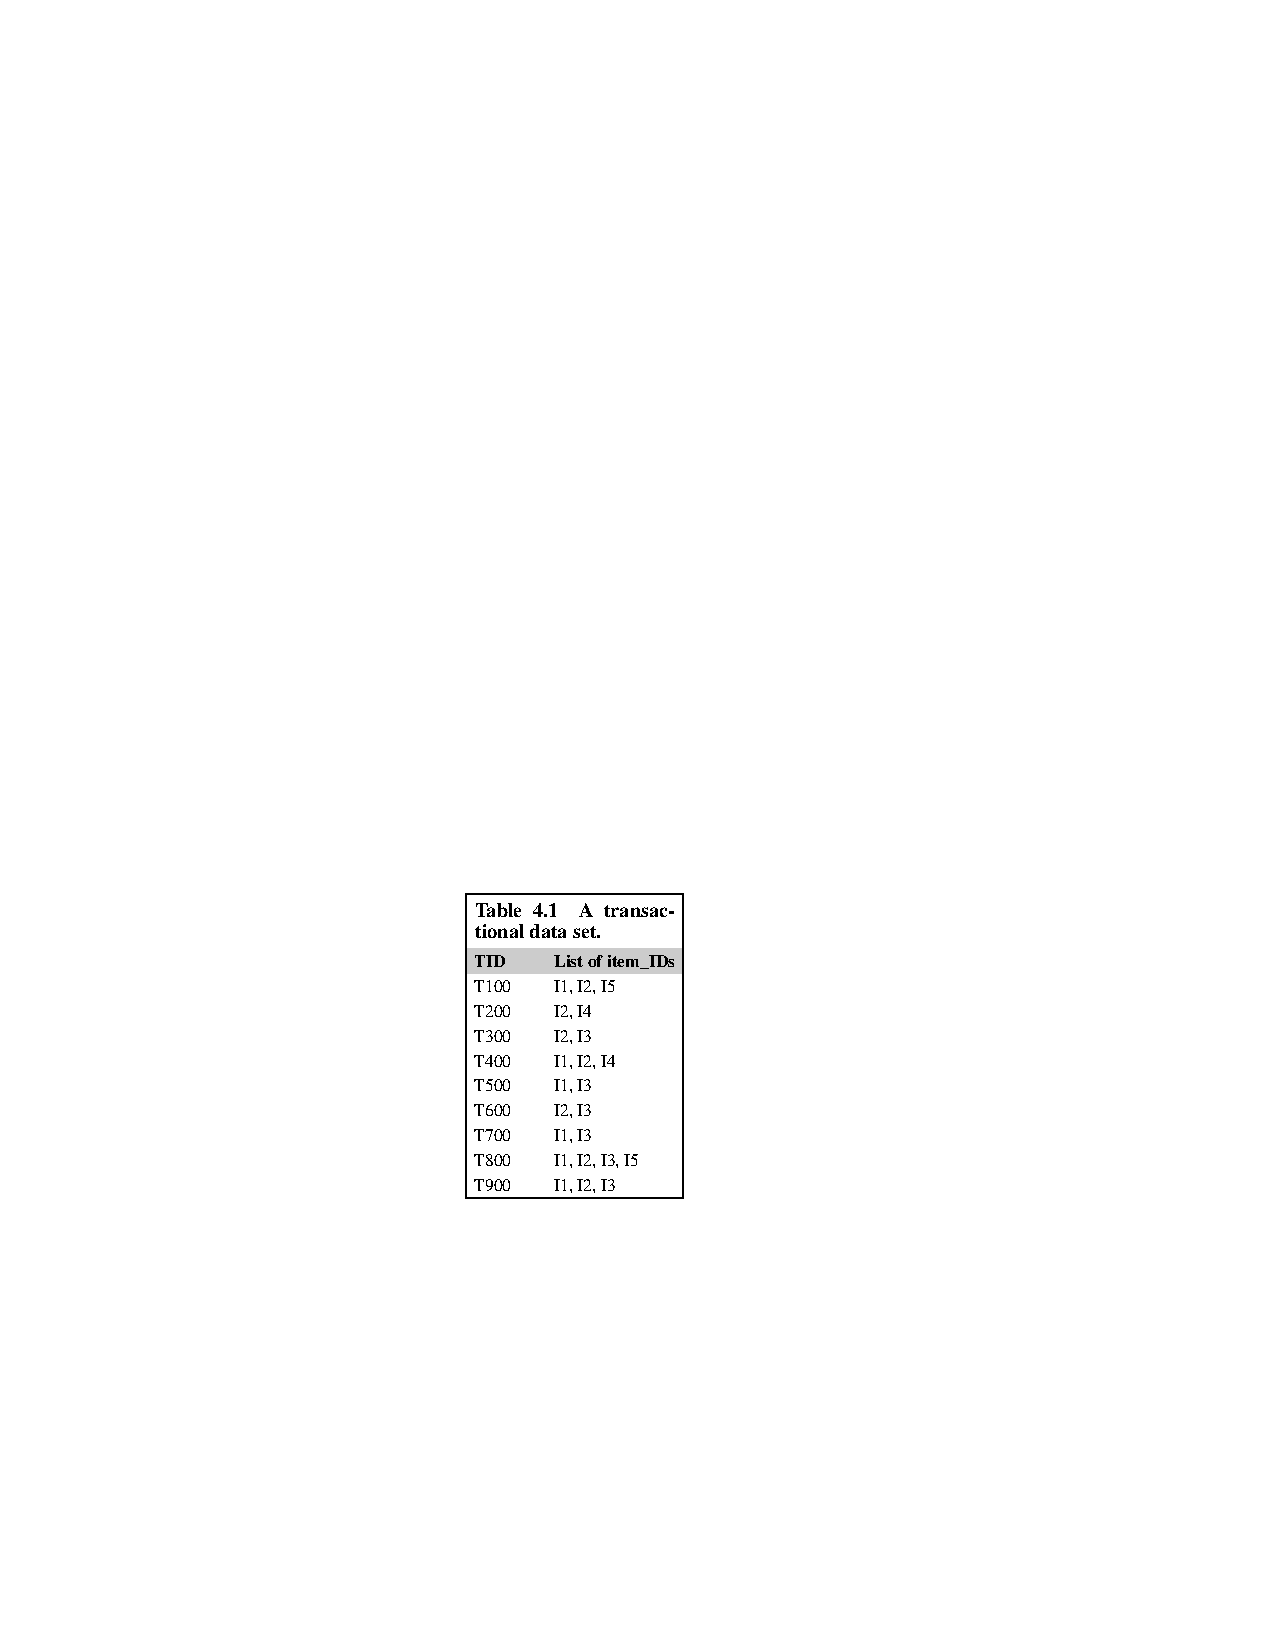
\includegraphics[height=0.8\textheight]{figures/4_3} \\
    \textbf{Database TDB} ($\text{minsup} = 2$)
\end{frame}

\begin{frame}{The Apriori Algorithm --An Example}
    \centering
    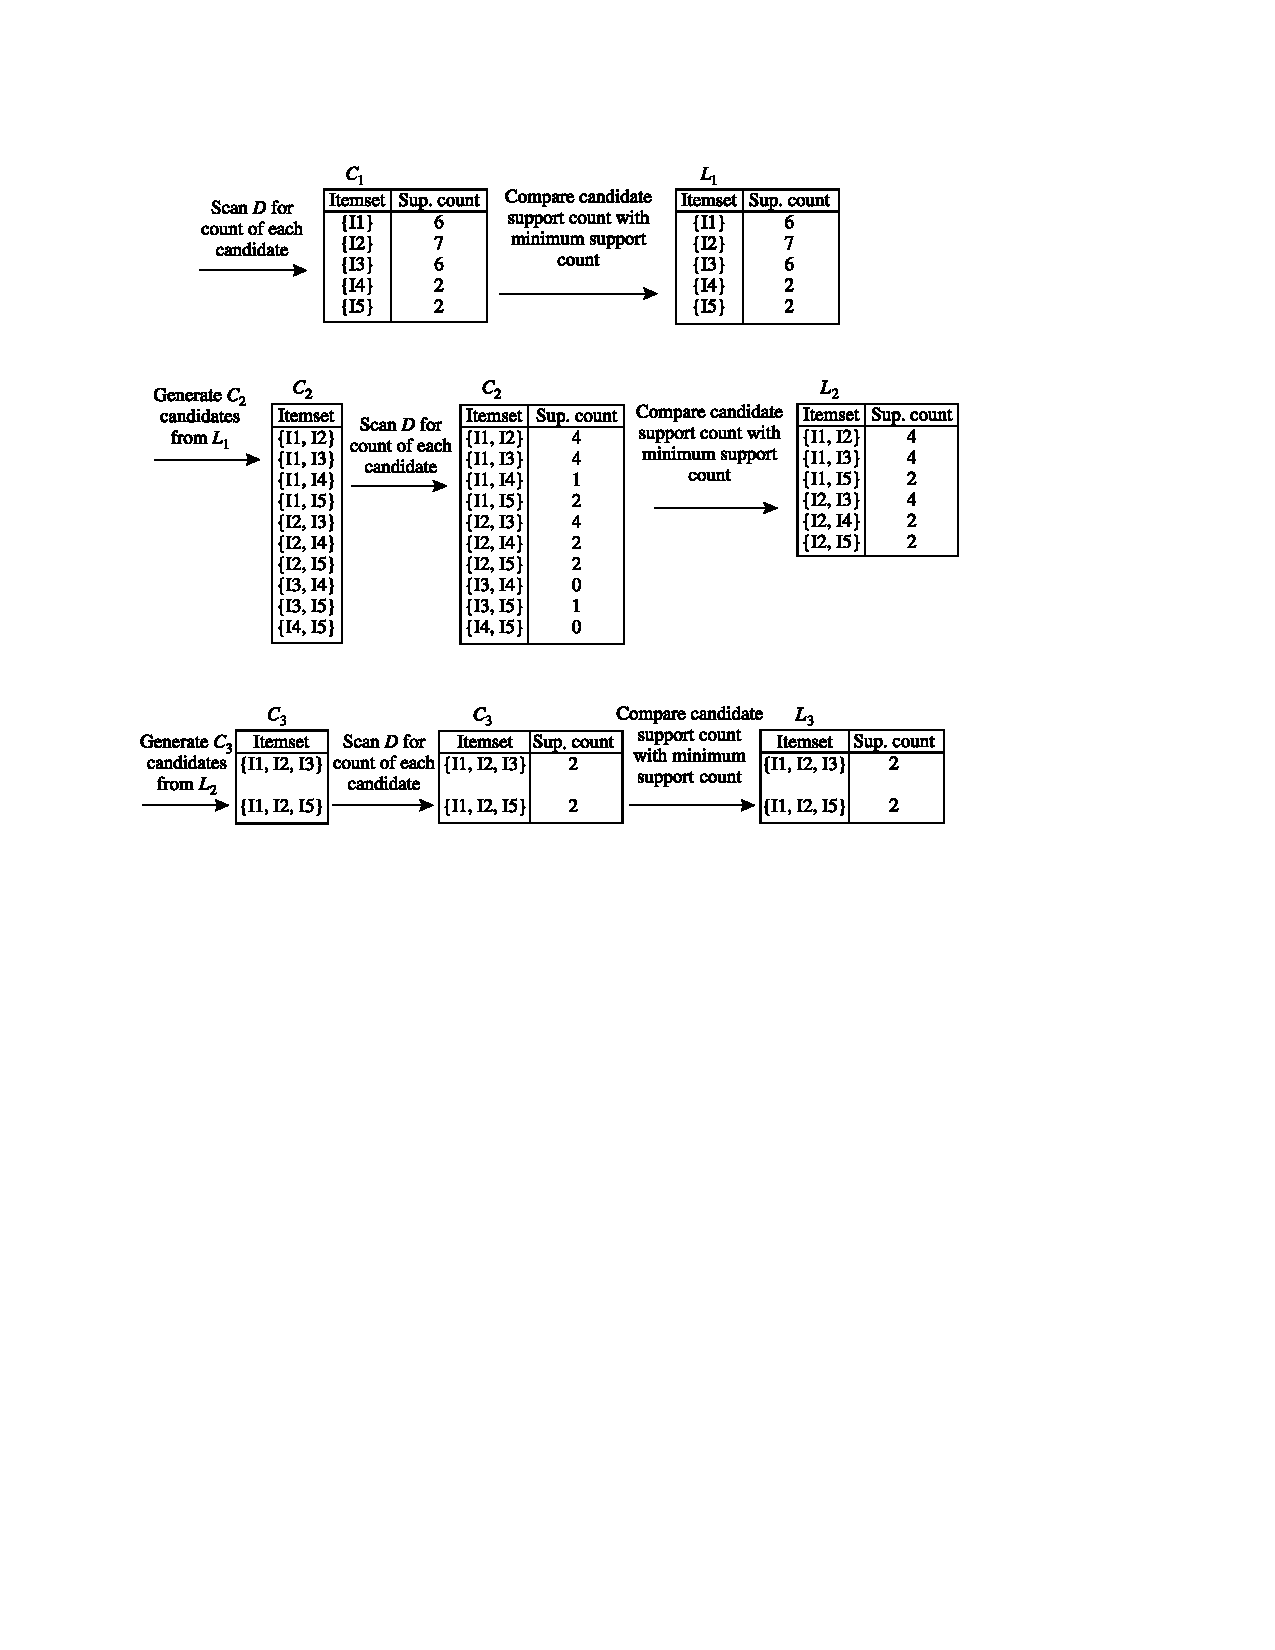
\includegraphics[height=0.9\textheight]{figures/4_4}
\end{frame}

\begin{frame}{Apriori: Improvements and Alternatives}
    \begin{itemize}
        \item \textbf{Reduce passes of transaction database scans}
        \begin{itemize}
            \item Partitioning (e.g., Savasere, et al., 1995) %\textit{[To be discussed in subsequent slides]}
            \item Dynamic itemset counting (Brin, et al., 1997)
        \end{itemize}
        \item \textbf{Shrink the number of candidates}
        \begin{itemize}
            \item Hashing (e.g., DHP: Park, et al., 1995) %\textit{[To be discussed in subsequent slides]}
            \item Pruning by support lower bounding (e.g., Bayardo, 1998)
            \item Sampling (e.g., Toivonen, 1996)
        \end{itemize}
        \item \textbf{Exploring special data structures}
        \begin{itemize}
            \item Tree projection (Agarwal, et al., 2001)
            \item H-miner (Pei, et al., 2001)
            \item Hypercube decomposition (e.g., LCM: Uno, et al., 2004)
        \end{itemize}
    \end{itemize}
\end{frame}

\subsection{FPGrowth}

\begin{frame}{Why Mining Frequent Patterns by Pattern Growth?}
    \begin{block}{Apriori: A breadth-first search mining algorithm}
        \begin{itemize}
            \item First find the complete set of frequent $k$-itemsets
            \item Then derive frequent $(k+1)$-itemset candidates
            \item Scan DB again to find true frequent $(k+1)$-itemsets
        \end{itemize}
    \end{block}
    \vspace{0.2cm}
    \begin{block}{Motivation for a different mining methodology}
        \begin{itemize}
            \item Can we develop a \textbf{depth-first search} mining algorithm?
            \item For a frequent itemset $\rho$, can subsequent search be confined to only those transactions containing $\rho$?
        \end{itemize}
    \end{block}
    \vspace{0.2cm}
    \begin{alertblock}{Such thinking leads to a frequent pattern growth approach: \textbf{FPGrowth}}
        \footnotesize FPGrowth (J. Han, J. Pei, Y. Yin, ``Mining Frequent Patterns without Candidate Generation,'' \textit{SIGMOD 2000})
    \end{alertblock}
\end{frame}

\begin{frame}{Example: From Transactional DB to Ordered Frequent Itemlist}

    \begin{columns}[T]
        % Left Column: Steps and Parameters
        \begin{column}{0.44\textwidth}
            \textbf{Let $\text{min\_support} = 3$}
            \vspace{0.2cm}
            \begin{itemize}
                \item \textbf{Scan DB once}, find single-item frequent patterns: \\
                \texttt{f:4, a:3, c:4, b:3, m:3, p:3}
                \vspace{0.15cm}
                \item \textbf{Sort frequent items} in frequency-descending order ($f$-list): \\
                \textbf{F-list = \texttt{f-c-a-b-m-p}}
                \vspace{0.15cm}
                \item \textbf{Scan DB again}, use the ordered frequent itemlist for each transaction to construct an FP-tree.
            \end{itemize}
        \end{column}

        % Right Column: Transactional Database Table
        \begin{column}{0.55\textwidth}
            \small
            \begin{tabular}{@{}lll@{}}
                \toprule
                             & \textbf{Items in}    & \textbf{Ordered Freq.} \\
                \textbf{TID} & \textbf{Transaction} & \textbf{Itemlist} \\
                \midrule
                100 & $\{f, a, c, d, g, i, m, p\}$ & $f, c, a, m, p$ \\
                200 & $\{a, b, c, f, l, m, o\}$    & $f, c, a, b, m$ \\
                300 & $\{b, f, h, j, o, w\}$       & $f, b$ \\
                400 & $\{b, c, k, s, p\}$          & $c, b, p$ \\
                500 & $\{a, f, c, e, l, p, m, n\}$ & $f, c, a, m, p$ \\
                \bottomrule
            \end{tabular}
            \vspace{4mm}
            \begin{block}{FP-Tree Construction:}
                For each transaction,insert the ordered frequent itemlist into an FP-tree,  with shared sub-branches merged, counts accumulated.
            \end{block}
        \end{column}
    \end{columns}
\end{frame}

\begin{frame}{Example: Construct FP-tree from Transaction DB}
    \centering
    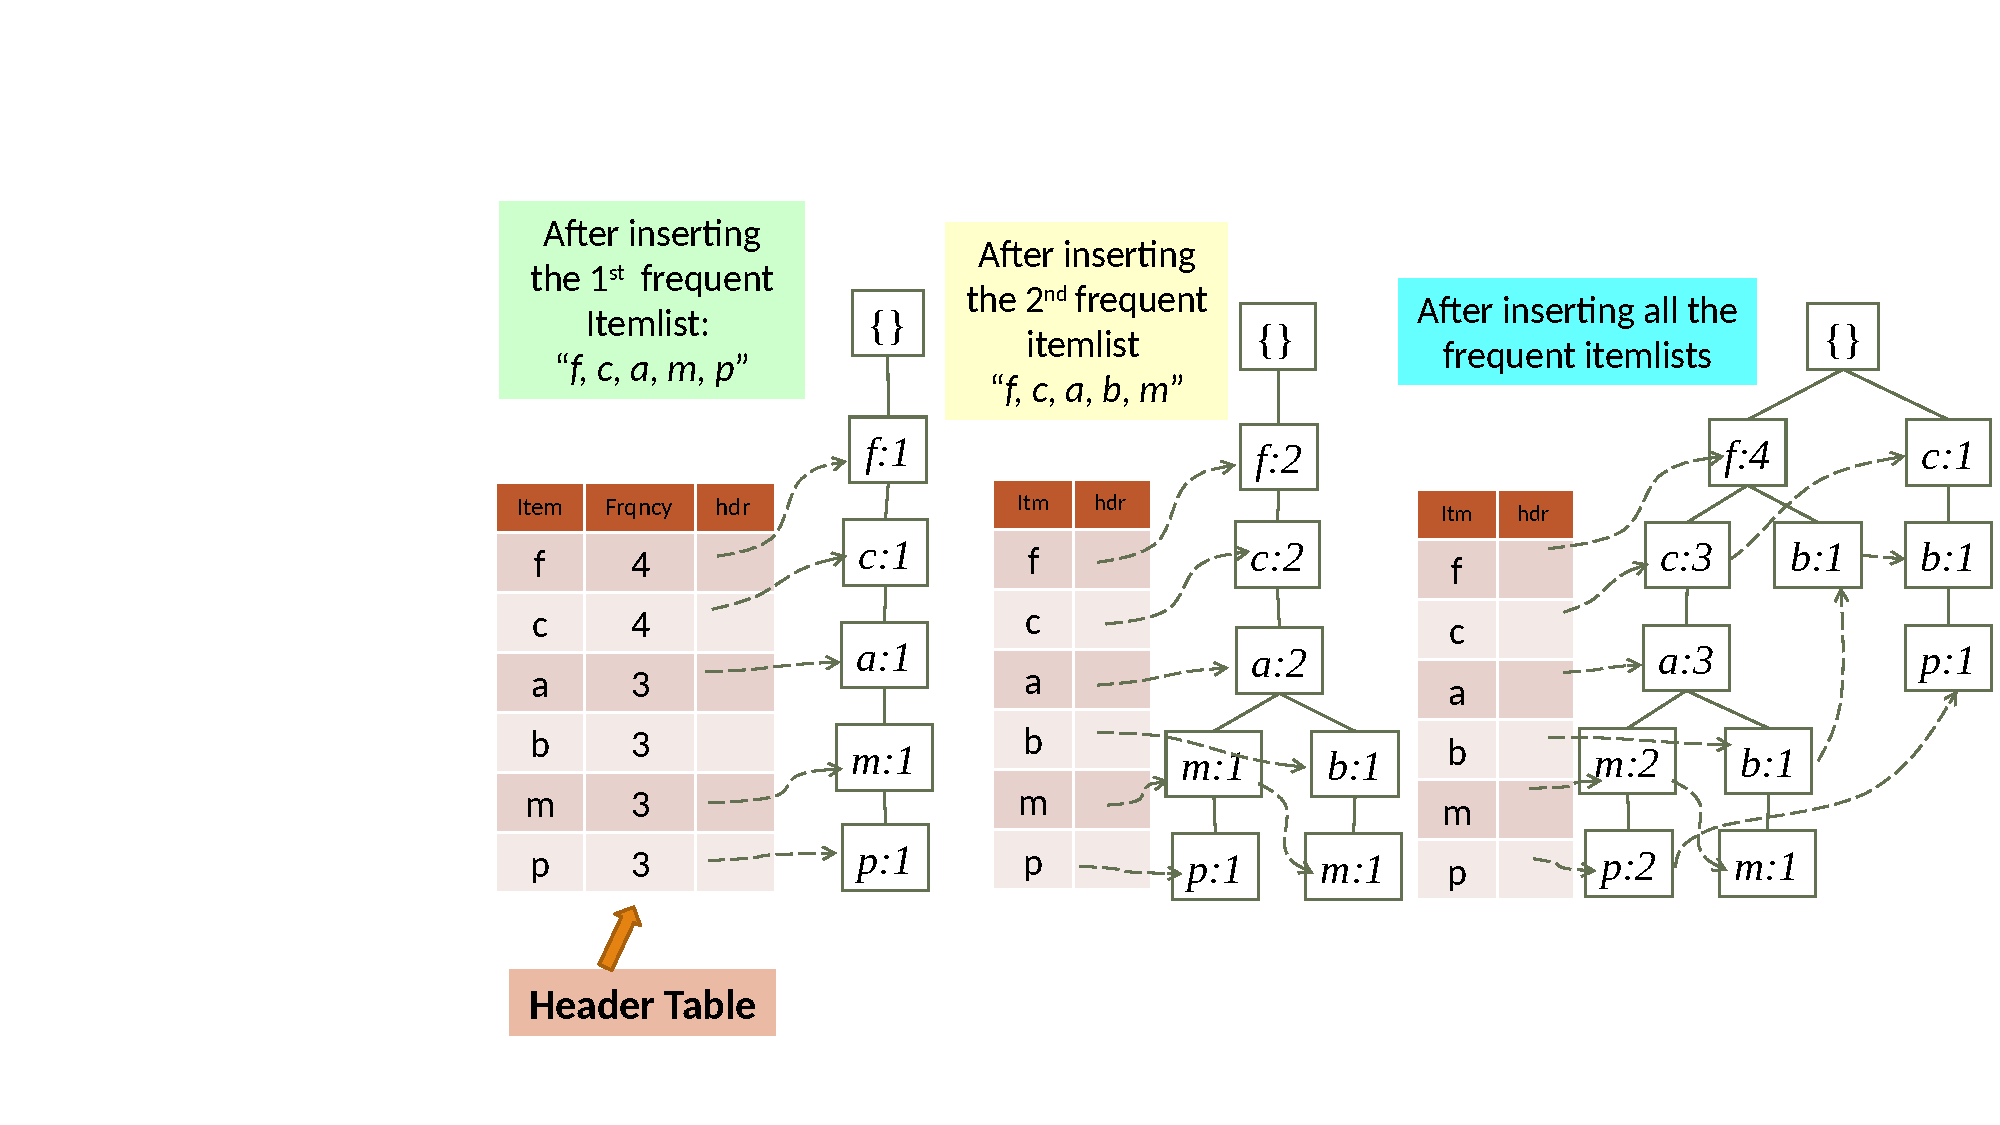
\includegraphics[width=\textwidth]{figures/4_5}
\end{frame}

\begin{frame}{Mining FP-Tree: Divide and Conquer Based on Patterns and Data}
    \centering
    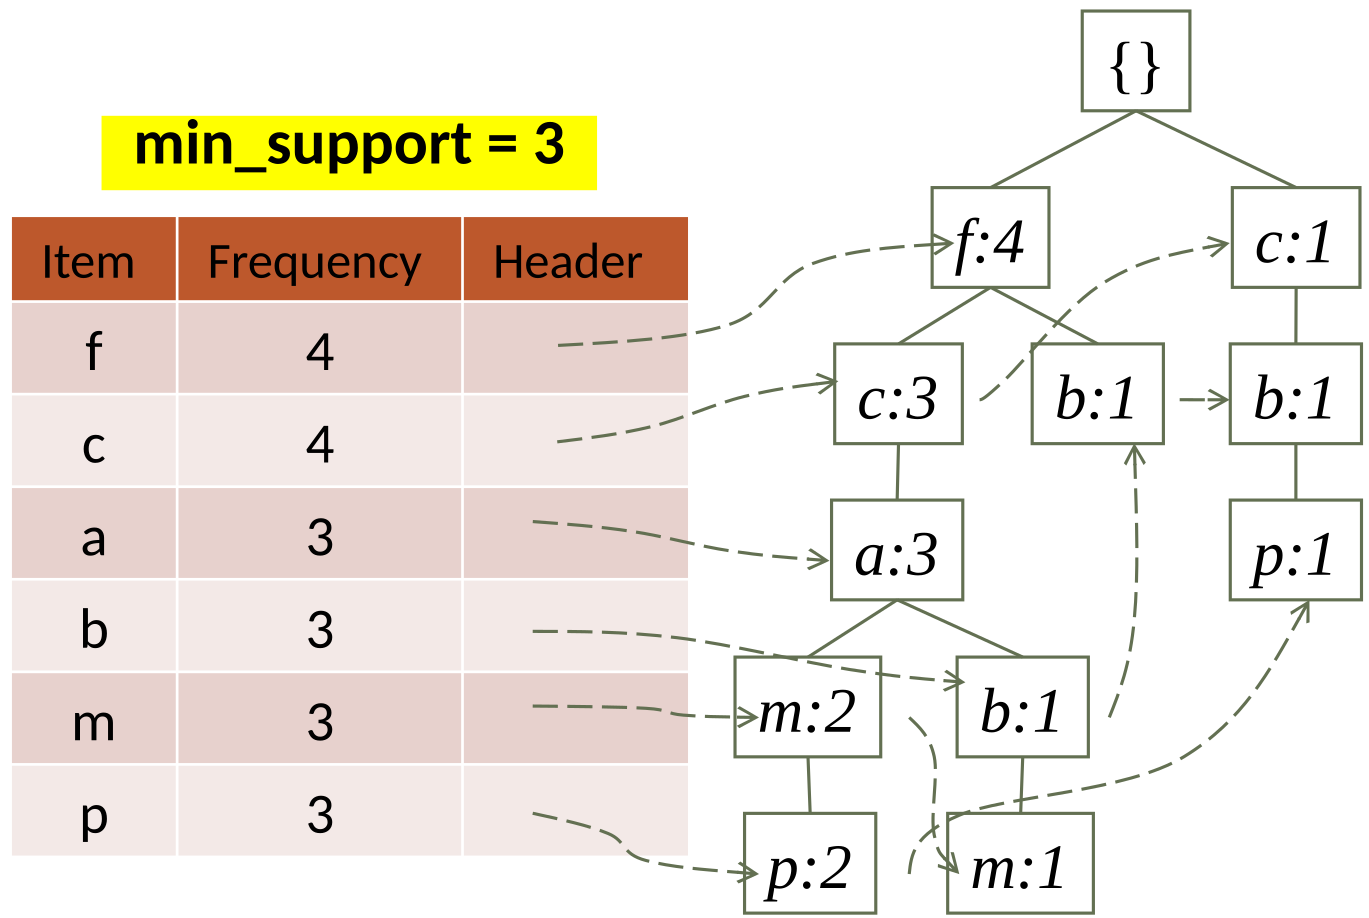
\includegraphics[width=0.475\textwidth]{figures/4_6} \\
    \begin{block}{Partitioning Pattern Mining}
        \begin{itemize}
            \item Pattern mining can be partitioned according to current patterns:
            \begin{itemize}
                \item \textbf{Patterns containing $p$:} $p$'s conditional database: \texttt{fcam:2, cb:1}
                \begin{itemize}
                    \item $p$'s conditional database (i.e., the database under the condition that $p$ exists):
                    \item \textit{transformed prefix paths of item $p$}
                \end{itemize}
                \item \textbf{Patterns having $m$ but no $p$:} $m$'s conditional database: \texttt{fca:2, fcab:1}
            \end{itemize}
        \end{itemize}
    \end{block}
\end{frame}

\begin{frame}{Mine Each Conditional Database Recursively}
    \begin{columns}[T]
        \begin{column}{0.39\textwidth}
            \begin{exampleblock}{$\text{min\_support} = 3$}
                \centering
                \begin{tabular}{@{}cl@{}}
                    \toprule
                                  & \textbf{Conditional} \\
                    \textbf{Item} & \textbf{Database} \\
                    \midrule
                    $c$ & \texttt{f:3} \\
                    $a$ & \texttt{fc:3} \\
                    $b$ & \texttt{fca:1, f:1, c:1} \\
                    $m$ & \texttt{fca:2, fcab:1} \\
                    $p$ & \texttt{fcam:2, cb:1} \\
                    \bottomrule
                \end{tabular}
            \end{exampleblock}
            \vspace{3mm}
            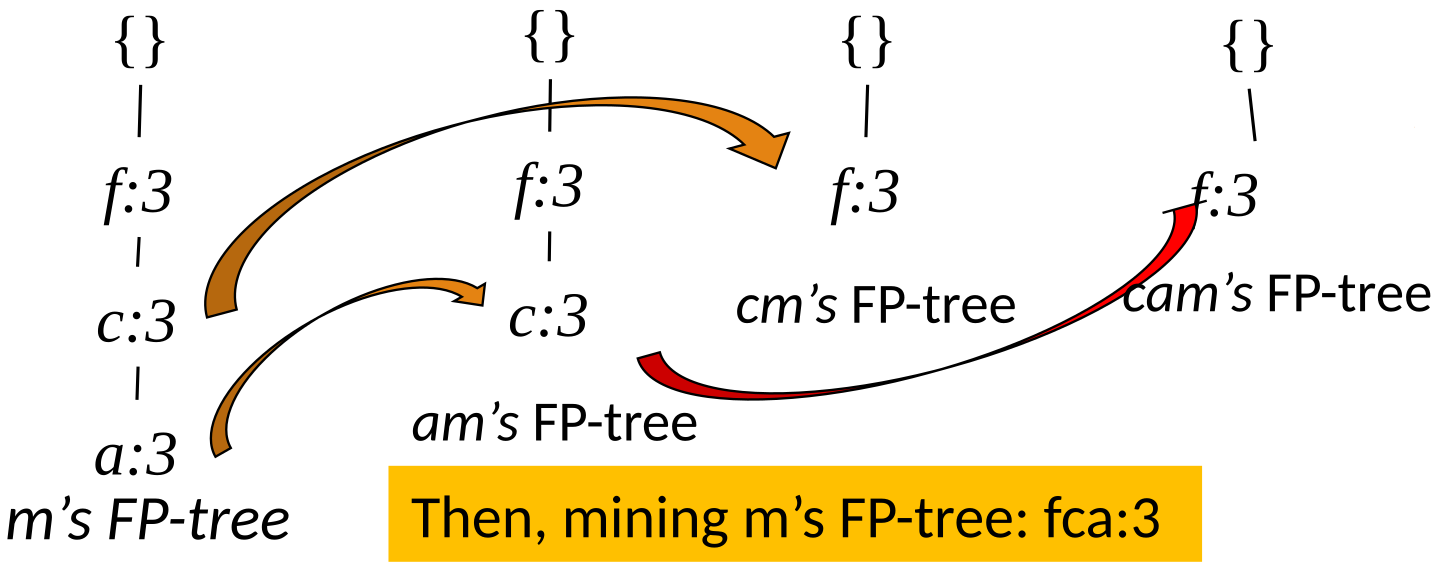
\includegraphics[width=\textwidth]{figures/4_7}
        \end{column}
        \begin{column}{0.60\textwidth}
            \begin{block}{For Each Conditional Database}
                \begin{itemize}
                    \item Mine single-item patterns
                    \item Construct its conditional FP-tree \& mine it
                \end{itemize}
            \end{block}
            \vspace{0.1cm}
            \begin{alertblock}{Conditional FP-Tree Results}
                \footnotesize
                \begin{itemize}
                    \item \textbf{$p$'s conditional DB:} \texttt{fcam:2, cb:1} $\rightarrow$ \texttt{c:3}
                    \vspace{0.15cm}
                    \item \textbf{$m$'s conditional DB:} \texttt{fca:2, fcab:1} $\rightarrow$ \texttt{fca:3}
                    \vspace{0.15cm}
                    \item \textbf{$b$'s conditional DB:} \texttt{fca:1, f:1, c:1} $\rightarrow \emptyset$
                \end{itemize}
                \textit{Actually, for single branch FP-tree, all the frequent patterns can be generated in one shot}
            \end{alertblock}
        \end{column}
    \end{columns}

\end{frame}

\begin{frame}{FPGrowth: Mining Frequent Patterns by Pattern Growth}
    \begin{block}{Essence of Frequent Pattern Growth (FPGrowth) Methodology}
        \begin{itemize}
            \item Find frequent single items and partition the database based on each such single-item pattern
            \item Recursively grow frequent patterns by doing the above for each partitioned database (also called the pattern's \textbf{conditional database})
            \item To facilitate efficient processing, an efficient data structure, \textbf{FP-tree}, can be constructed
        \end{itemize}
    \end{block}
    \vspace{2mm}
    \begin{alertblock}{Mining Process}
        \begin{itemize}
            \item \textbf{Recursively construct and mine} (conditional) FP-trees
            \item \textbf{Termination condition:} Until the resulting FP-tree is empty, or until it contains only \textbf{one path}, a single path will generate all the combinations of its sub-paths, each of which is a frequent pattern
        \end{itemize}
    \end{alertblock}
\end{frame}

\section{Which Patterns Are Interesting? Pattern Evaluation Methods}

\begin{frame}{How to Judge if a Rule/Pattern Is Interesting?}
    \begin{alertblock}{The Challenge}
        \begin{itemize}
            \item Pattern-mining will generate a large set of patterns/rules
            \item \textbf{Not all} the generated patterns/rules are interesting
        \end{itemize}
    \end{alertblock}
    \vspace{0.2cm}
    \begin{block}{Interestingness Measures: Objective vs. Subjective}
        \begin{columns}[T]
            % Left Column: Objective Measures
            \begin{column}{0.46\textwidth}
                \textbf{Objective Interestingness Measures}
                \begin{itemize}
                    \item Data-driven statistical metrics:
                    \begin{itemize}
                        \item Support
                        \item Confidence
                        \item Correlation, \dots
                    \end{itemize}
                \end{itemize}
            \end{column}
            % Right Column: Subjective Measures
            \begin{column}{0.50\textwidth}
                \textbf{Subjective Interestingness Measures}
                \begin{itemize}
                    \item Different users may judge interestingness differently
                    \item Let a user specify:
                    \begin{itemize}
                        \item \textbf{Query-based:} Relevant to a user's particular request
                        \item \textbf{Against knowledge-base:} Unexpected, freshness, timeliness
                    \end{itemize}
                \end{itemize}
            \end{column}
        \end{columns}
    \end{block}
\end{frame}

\begin{frame}{Limitation of the Support-Confidence Framework}
    \begin{alertblock}{Are $s$ and $c$ interesting in association rules: ``$A \Rightarrow B$'' $[s, c]$?}
        \textbf{Be careful!} High support and confidence can still produce misleading rules.
    \end{alertblock}
    \vspace{0.1cm}
    \begin{exampleblock}{Example: School Student Statistics}
        \centering
        \footnotesize
        \begin{tabular}{@{}lccc@{}}
            \toprule
            & \textbf{play-bball} & \textbf{not play-bball} & \textbf{sum (row)} \\
            \midrule
            \textbf{eat-cereal}     & 400 & 350 & 750 \\
            \textbf{not eat-cereal} & 200 & 50  & 250 \\
            \midrule
            \textbf{sum (col.)}     & 600 & 400 & 1000 \\
            \bottomrule
        \end{tabular}
    \end{exampleblock}
    \begin{block}{Association Rule Analysis}
        \footnotesize
        \begin{itemize}
            \item \textbf{Generated Rule:} $\text{play-basketball} \Rightarrow \text{eat-cereal}\ [40\%, 66.7\%]$ \textit{(higher $s$ \& $c$)}
            \item \textbf{Why it is misleading:} Overall $\%$ of students eating cereal is $\mathbf{75\% > 66.7\%}$ (playing basketball actually lowers the likelihood!).
            \item \textbf{A more telling rule:} $\neg\text{play-basketball} \Rightarrow \text{eat-cereal}\ [35\%, 87.5\%]$ \textit{(high $s$ \& $c$)}
        \end{itemize}
    \end{block}
\end{frame}

\begin{frame}{Interestingness Measure: Lift}
    \begin{columns}[T]
        \begin{column}{0.49\textwidth}
            \footnotesize
            \begin{block}{Measure of Dependent/Correlated Events}
                \[
                    \text{lift}(B, C) = \frac{c(B \rightarrow C)}{s(C)} = \frac{s(B \cup C)}{s(B) \times s(C)}
                \]
            \end{block}
            \vspace{0.1cm}
            \begin{block}{Lift(B, C) may tell how $B$ and $C$ are correlated}
                \begin{itemize}
                    \item $\text{lift}(B, C) = 1$: $B$ and $C$ are \textbf{independent}
                    \item $\text{lift}(B, C) > 1$: \textbf{positively} correlated
                    \item $\text{lift}(B, C) < 1$: \textbf{negatively} correlated
                \end{itemize}
            \end{block}
        \end{column}
        \begin{column}{0.49\textwidth}
            \footnotesize
            \begin{exampleblock}{For Our Example ($B$: basketball, $C$: cereal)}
                \vspace{-0.2cm}
                \begin{align*}
                    \text{lift}(B, C) &= \frac{400 / 1000}{(600 / 1000) \times (750 / 1000)} = \mathbf{0.89} \\[0.2cm]
                    \text{lift}(B, \neg C) &= \frac{200 / 1000}{(600 / 1000) \times (250 / 1000)} = \mathbf{1.33}
                \end{align*}
            \end{exampleblock}
            \vspace{0.1cm}
            \begin{alertblock}{Conclusion}
                \footnotesize
                \begin{itemize}
                    \item $B$ and $C$ are \textbf{negatively correlated} since $\text{lift}(B, C) < 1$
                    \item $B$ and $\neg C$ are \textbf{positively correlated} since $\text{lift}(B, \neg C) > 1$
                \end{itemize}
            \end{alertblock}
        \end{column}
    \end{columns}
\end{frame}

%%%%%%%%%%%%%%%%%%%%%%%%%%%%%%%%%%%%%%%%%%%%%%%%%%%%%%%%%%%%%%%%%%%%%%%%%
\begin{frame}{}
    \centering
    \Huge End of Chapter 4.
\end{frame}

\begin{frame}{Data Mining: Concepts and Techniques}
    \centering
    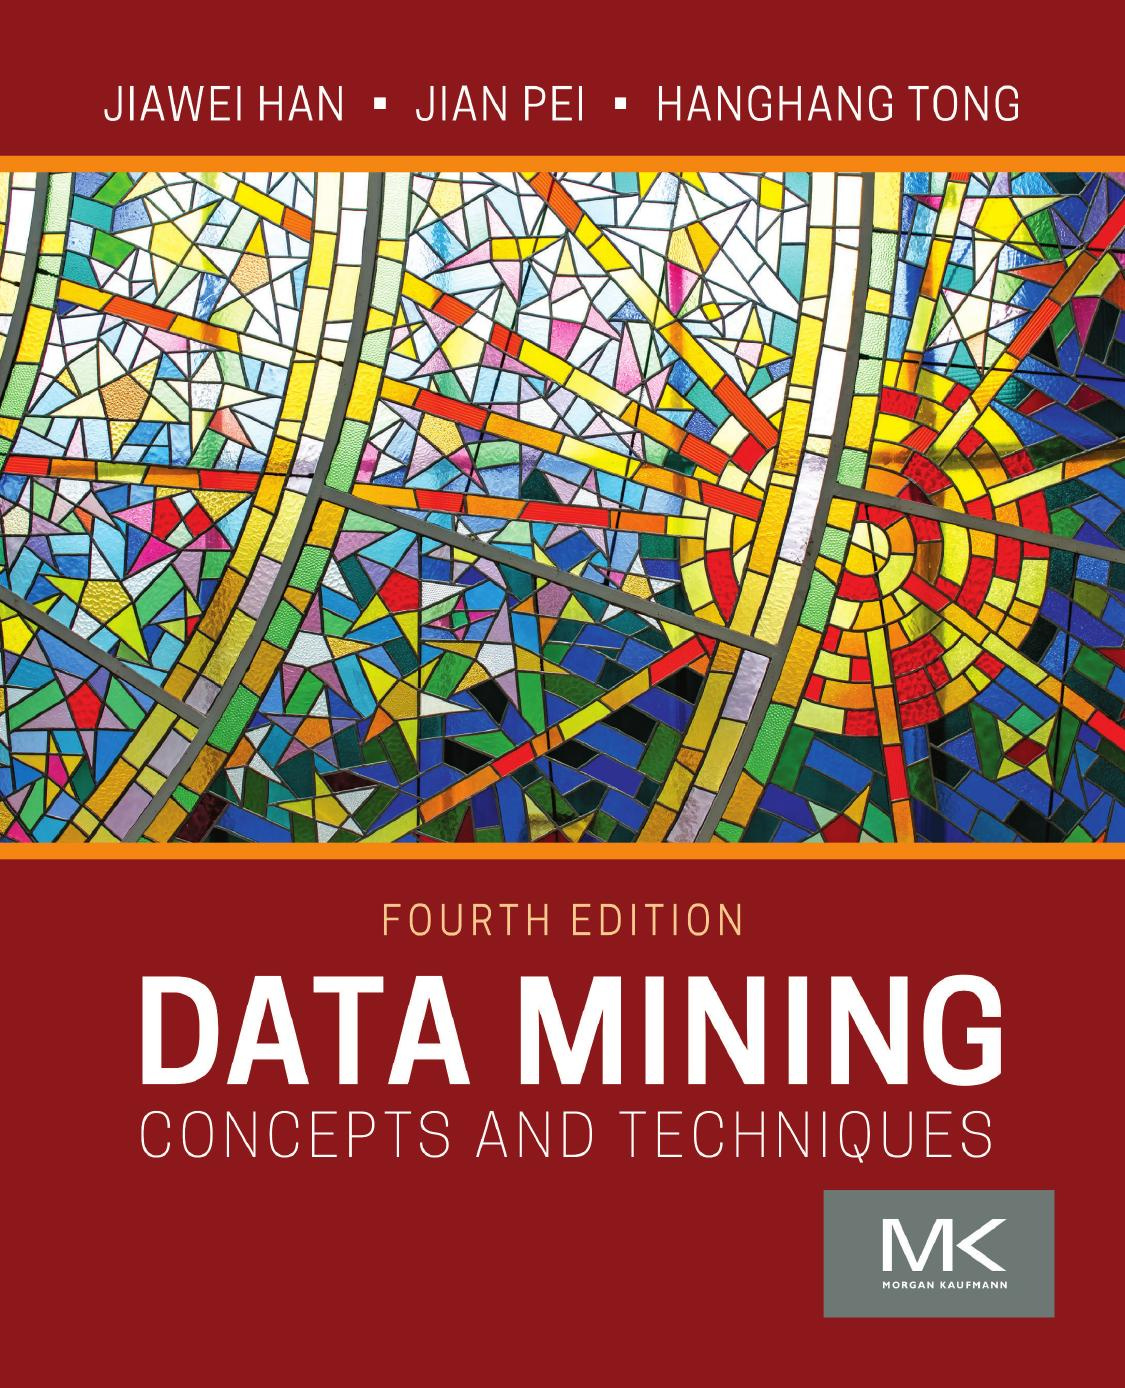
\includegraphics[height=0.7\textheight]{figures/cover} \\
    \vspace{4mm}
    {
        \tiny
        Content has been extracted from \textit{Data Mining: Concepts and Techniques}, Fourth Edition, by Jiawei Han, Jian Pei \& Hanghang Tong. Morgan Kaufmann Publishers. 2023.\\
        Visit \url{https://hanj.cs.illinois.edu/bk4/}.\\
    }
\end{frame}

\end{document}
